
\section{Segmentations}

\begin{frame}
  \frametitle{Segmentations}
 
  \begin{block}{Definition}
A segmentation is an \emph{ordered} set of segments (of a same class) \emph{spanning} a given range. 

~

A given range contains a finite set of segments of a given class. 
A segmentation is a subset of the whole set of segments such that:
\begin{enumerate}
 \item (spanning) each element of the range belongs to a segment of the subset
 \item (ordered) no segment contains another segment of the subset 
\end{enumerate}
Due to (2), the segments of a segmentation can be ordered without ambiguity 
(according to the relative position of their first element for instance).
  \end{block}

%  \begin{block}{Main type}
%SegmentComputerIterator
% \begin{itemize}
%  \item dereference operator: return an instance of a segment computer.
%  \item intersectPrevious(), intersectNext(): return 'true' if the current segment intersects, respectively, the %previous and the next one (when they exist), 'false' otherwise.
% \end{itemize}
%  \end{block}

 % \begin{block}{Main method}
%init method taking as input parameters: 
%\begin{itemize}
% \item begin/end (circular)iterators of the range to be segmented
% \item an instance of segment computer
%\end{itemize}
%  \end{block}

 \begin{center}
   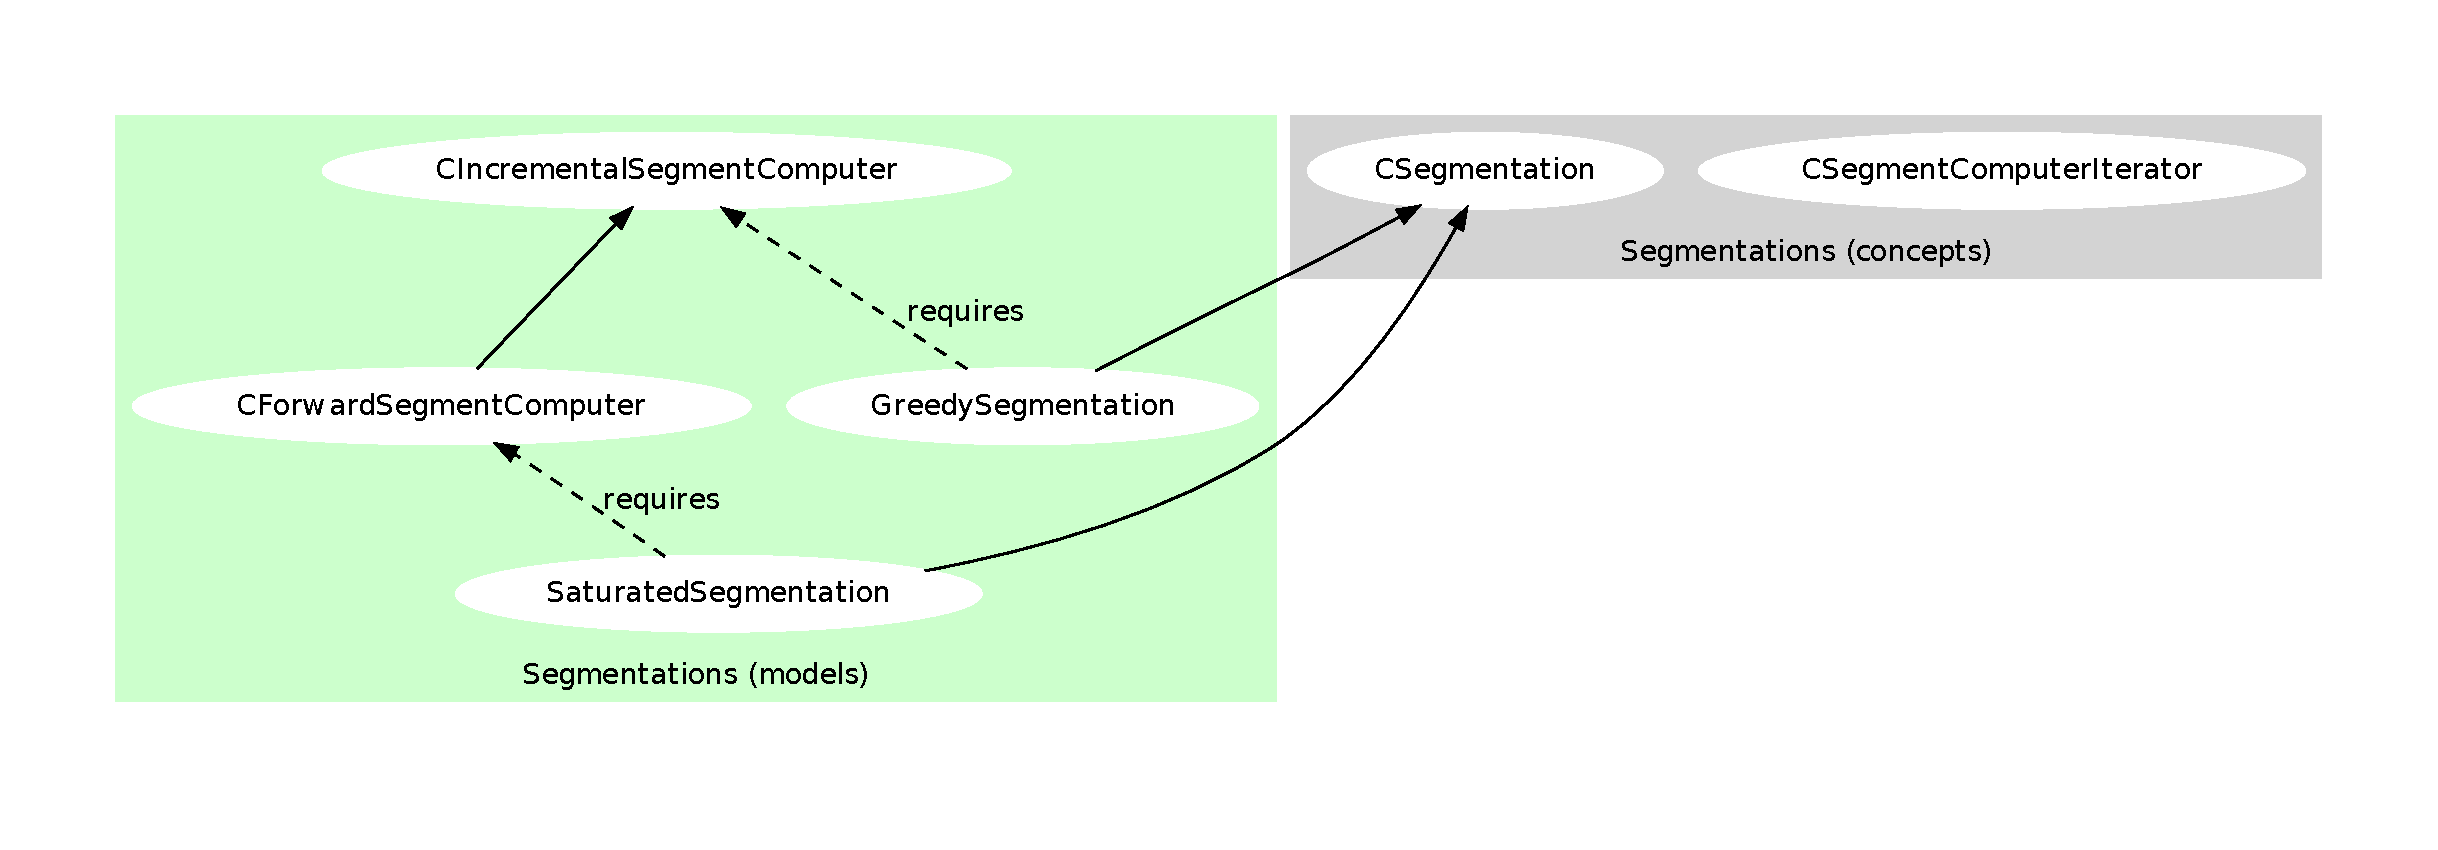
\includegraphics[width=1\textwidth]{segmentationsGraph}
 \end{center}

\end{frame}


\begin{frame}[containsverbatim]
  \frametitle{Example: greedy segmentation into DSS}

  \begin{lstlisting}
  ... // Let r be a range of type Range;

  //types
  typedef ArithmeticalDSS<Range::ConstIterator> SegmentComputer;
  typedef GreedySegmentation<SegmentComputer> Segmentation;

  //instances
  SegmentComputer detectionAlgorithm;
  Segmentation theSegmentation(r.begin(), r.end(), detectionAlgorithm);
                                 
  typedef Segmentation::SegmentComputerIterator SCIterator;  
  SCIterator it = theSegmentation.begin();
  SCIterator itEnd = theSegmentation.end();
  for ( ; it != itEnd; ++it) 
    {
     SegmentComputer current(*it);
     ...
    }
  \end{lstlisting}

 \begin{center}
   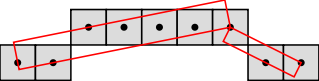
\includegraphics[width=0.45\textwidth]{left_right}
 \end{center}

\end{frame}


\begin{frame}[containsverbatim]
  \frametitle{Other segmentations}

  \begin{lstlisting}
...
  typedef ArithmeticalDSS<Range::ConstReverseIterator> SegmentComputer;
...
  Segmentation theSegmentation(r.rbegin(), r.rend(), detectionAlgorithm);
...
  \end{lstlisting}

 \begin{center}
   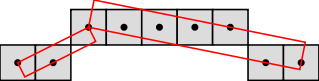
\includegraphics[width=0.45\textwidth]{right_left}
 \end{center}

  \begin{lstlisting}
...
   typedef SaturatedSegmentation<SegmentComputer> Segmentation;
...
  \end{lstlisting}

 \begin{center}
   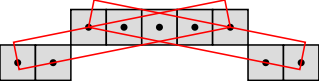
\includegraphics[width=0.45\textwidth]{maxseg}
 \end{center}

\end{frame}

\begin{frame}[fragile]
  \frametitle{Segmentation of subranges}

  \begin{verbatim}
theSegmentation.setSubRange(beginIt, endIt);
theSegmentation.setMode("myMode");
  \end{verbatim}

\begin{itemize}
 \item GreedySegmentation
  \begin{itemize}
   \item \alert<1>{"Truncate" (default)}
   \item "Truncate+1"
   \item "DoNotTruncate"
  \end{itemize}
 \item SaturatedSegmentation
  \begin{itemize}
   \item "First",
   \item \alert<2>{"MostCentered" (default)}
   \item "Last"
  \end{itemize}
\end{itemize}

\only<1>{
\begin{center}
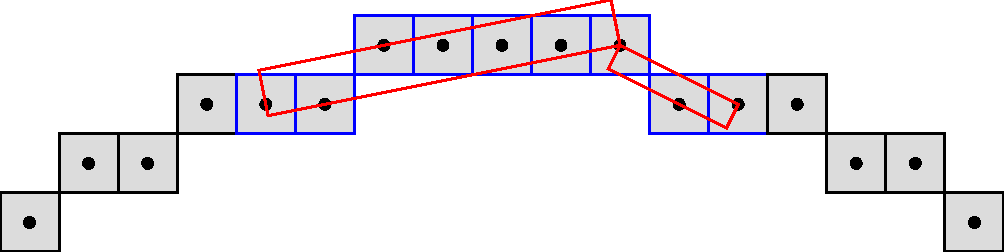
\includegraphics[height=0.2\textheight]{greedyseg-Truncate}
\end{center}
}
\only<2>{
\begin{center}
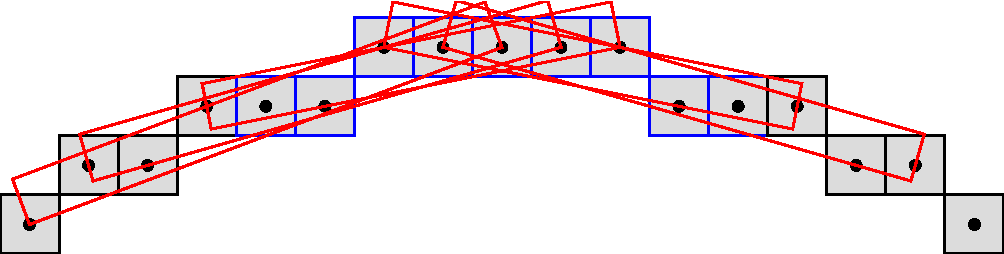
\includegraphics[height=0.2\textheight]{saturatedseg-MostCentered}
\end{center}
}

%NB: a whole range in a closed/circular structure 
%may be viewed as a subrange of a periodic signal. 
\end{frame}

\begin{frame}
  \frametitle{Done (red) and to do (black)}
 

\begin{block}{Segment computers}
\begin{itemize}
  \item \alert{ArithmeticalDSS}
  \item \alert{ArithmeticalDSS3d} (I. Sivignon)
  \item \alert{CombinatorialDSS} (X. Proven\c{c}al)
  \item \alert{GeometricalDSS}
  \item \alert{GeometricalDCA}
  \item ThickSegment
  \item ConvexPart
  \item other based on linear programming
\end{itemize}
\end{block}

\begin{block}{Segmentations}
\begin{itemize}
  \item \alert{GreedySegmentation}: with overlapping at one point (for polygonalisations)
  \item greedy segmentation without overlapping (to get a partition)
  \item greedy segmentation into a minimal number of segments for closed structures 
  \item \alert{SaturatedSegmentation}: all maximal segments
  \item segmentation into a minimal number of \emph{maximal} segments
  \item pencil structure (all segments intersecting at a given element)
\end{itemize}
\end{block}

\end{frame}

\begin{frame}[squeeze]
  \frametitle{Module description (as of 0.5)}

  \begin{block}{Content}
    \begin{itemize}
      \small
    \item One data structure based on a cellular grid space (GridCurve),
    \item which provides different views of the same digital curve (XXXRange).
    \item A segmentation framework (concepts of segment computers and segmentations).
    \item Many detection algorithms (models of segment computers).
    \end{itemize}
  \end{block}

  \begin{block}{Examples}
    \begin{itemize}
      \small
    \item GridCurve (d=1,n=2), (d=1,n=3), (d=2,n=3)
    \item Greedy/Saturated segmentation of (sub)ranges
    \item ArithmeticalDSS(3d)/CombinatorialDSS/GeometricalDSS, GeometricalDCA
    \item convex and concave parts
    \end{itemize}
  \end{block}

  \begin{block}{Location}
    \begin{itemize}
    \item \texttt{\{DGtal\}/src/DGtal/base} (Iterator/Range stuffs)
    \item \texttt{\{DGtal\}/src/DGtal/geometry/curves/representation} (Geometry part) 
    \item \texttt{\{DGtal\}/tests/geometry/curves/representation}
    \item \texttt{\{DGtal\}/examples/geometry/curves/representation}
    \end{itemize}
  \end{block}

\end{frame}
